\chapter{Divergences, Propagators, and the Supersymmetric Motive}

This lecture was supposed to begin supersymmetry itself. Instead, it does something more deliberate: it backs up and rebuilds the need for supersymmetry from the problem of ultraviolet divergences, especially the renormalization of masses. That is the right order. Before we talk about a powerful new symmetry, we should understand what sort of damage needs repairing. The chapter therefore unfolds in the same order as the lecture: first effective Lagrangians and propagators, then the short-distance behavior of scalar and fermion fields, then the simplest divergent loop corrections, and only at the end the first real glimpse of what supersymmetry is supposed to accomplish.

\section{Why We Are Still Talking About Divergences}

A great deal of particle physics is the computation of Feynman diagrams. To say that, however, is not yet to say what Feynman diagrams are for. The lecture begins by reminding us that they serve at least two rather different purposes.

First, they compute scattering amplitudes. Particles come in, particles go out, and we sum the diagrams that contribute to the probability amplitude. Second, and for the present lecture more importantly, they help us construct an effective Lagrangian. In that setting the point is not to write the exact microscopic theory in a different notation. The point is to write an approximate theory that is effective because it has been stripped of short-distance complications that we do not yet know how to calculate.

That is why a cutoff enters almost immediately. An effective Lagrangian is typically accompanied by either
\begin{itemize}
\item a smallest distance, or
\item a largest momentum.
\end{itemize}
The lecture keeps both descriptions alive from the start, because the same ultraviolet problem will soon be read in both languages.

\section{Propagators in Position Space and Momentum Space}

The propagator is the bridge between those two descriptions. If a particle is inserted at one spacetime point and later detected at another, the corresponding amplitude depends on the separation between the two points. To keep the notation unambiguous on the page, we shall write
\begin{equation}
\Delta^\mu = y^\mu - x^\mu
\end{equation}
for the spacetime separation, reserving \(\delta\) for the ultraviolet cutoff length.

For a scalar field, the propagator is used in the lecture schematically as both an amplitude from \(x\) to \(y\) and as a vacuum expectation value:
\begin{equation}
G_\phi(x,y) \sim \langle 0 | \phi(x)\phi(y) |0\rangle .
\end{equation}
The exact time-ordering conventions are not the point here. What matters is that the propagator depends on \(x\) and \(y\) only through their difference.

Now the lecture makes a move that is conceptually simple but structurally crucial. A closed loop may be regarded in either of two ways:
\begin{itemize}
\item as a propagator from a point back to itself;
\item as an integral over all momentum that can circulate around the loop.
\end{itemize}
That is the same diagram seen from position space and momentum space. Once one sees this, the later discussion of divergences becomes almost inevitable.

\subsection{Question \& Answer}

\textbf{Question.} Why are short-distance divergences the same thing as high-momentum divergences?

\textbf{Answer.} Because momentum is inverse wavelength. Very large momentum means very short wavelength, and very short wavelength means very fine spatial resolution. Thus a singularity when \(\Delta \to 0\) in position space is the same ultraviolet phenomenon as a divergence from integrating over arbitrarily large loop momentum in momentum space. The lecture insists on this early because every later estimate can be translated back and forth between the two pictures.

\section{Scalar Fields, Dimensional Analysis, and the Massless Propagator}

Having set up the general language, the lecture narrows to the first case that matters physically here: scalar fields. There are not many fundamental scalars in particle physics, but the Higgs boson is enough to make the problem urgent.

The argument begins in a very characteristic way: before computing anything in detail, let us ask what dimensional analysis already forces on us. For a scalar field \(\phi\), the simplest action is
\begin{equation}
S_\phi \sim \int d^4x\, (\partial_\mu \phi)^2 .
\end{equation}
The exact normalization is not important for the present argument. What matters is that in units with \(\hbar=c=1\), the action is dimensionless. Therefore
\begin{align}
1 &\sim [S_\phi]
   \sim [d^4x]\,[\partial_\mu\phi]^2 \\
  &\sim L^4 \left(L^{-1}[\phi]\right)^2 .
\end{align}
Hence
\begin{equation}
[\phi]=L^{-1}.
\end{equation}

The lecture then checks the other familiar terms one by one. If we add a mass term \(m^2\phi^2\), dimensional consistency requires
\begin{equation}
[m]=L^{-1}.
\end{equation}
If we add a quartic interaction \(\lambda \phi^4\), then
\begin{equation}
[\lambda]=L^0,
\end{equation}
so the quartic scalar coupling is dimensionless in four dimensions.

Now let us return to the propagator. In the massless case there is no scale in the problem other than the separation \(\Delta\). Translation invariance says that the propagator depends only on \(x-y\), Lorentz invariance says that it depends only on the invariant interval, and dimensional analysis says that it must carry the dimensions of two scalar fields. There is therefore essentially no choice:
\begin{equation}
G_\phi(\Delta)\propto \frac{1}{\Delta^2},
\qquad
\Delta^2=\Delta_\mu\Delta^\mu .
\end{equation}
Numerical factors are present, but no new scale is.

The lecture then asks what happens when the field has a mass. The point is not to write the exact massive propagator. The point is to understand its short-distance behavior. For this the dispersion relation is enough:
\begin{equation}
E=\sqrt{p^2+m^2},
\qquad
E=|p|
\quad \text{for a massless particle.}
\end{equation}
When \(|p|\gg m\), the massive expression forgets the mass and approaches the massless one. Large momentum means short distance, so the short-distance propagator must likewise forget the mass.

At larger separations the mass suppresses propagation. The lecture writes this schematically as an exponential cutoff, so one may think of the massive scalar propagator as behaving roughly like
\begin{equation}
G_{\phi,m}(\Delta)\approx \frac{1}{\Delta^2}e^{-m|\Delta|}.
\end{equation}
This should be read as a guide, not an exact formula. Its purpose is to make one point clear: at large separation the mass matters, but near \(\Delta=0\) the singularity is still the same \(1/\Delta^2\).

\section{The Simplest Scalar Self-Energy Diagram and the Fine-Tuning Problem}

Now the lecture cashes out all of this preparatory work. We turn from the abstract question ``what does a propagator look like?'' to the concrete question ``what does the simplest loop correction do to a scalar mass?''

The preserved blackboard frame is useful here because it shows the transition exactly as it happened in the lecture: the earlier discussion has not yet disappeared. One still sees the relativistic energy formula, its massless limit, part of the scalar-field action, and now in the middle the simplest loop correction.

\begin{figure}[t]
\centering

\includegraphics[width=0.82\textwidth]{lecture_03_figure_02.png}
\caption{Blackboard moment at the transition from propagators and dimensional analysis to the simplest loop correction. The visible kinematic formulas and the partly visible action term are part of the same chain of reasoning as the loop diagram in the middle.}
\end{figure}

Cleaned up, and with the partly visible action term written in the standard form suggested by the immediately preceding discussion, the board content may be summarized schematically as
\begin{equation}
E=\sqrt{p^2+m^2},
\qquad
E=|p|,
\qquad
S_\phi \sim \int d^4x\,(\partial_\mu\phi)^2,
\qquad
[\phi]=L^{-1}.
\end{equation}
So the loop diagram is not appearing from nowhere. It is the direct consequence of what we have just learned about short-distance propagation.

\begin{figure}[t]
\centering
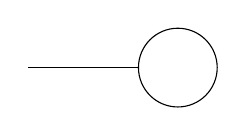
\begin{tikzpicture}[scale=1.0]
\draw (-2.0,0) -- (-0.6,0);
\draw (-0.1,0) circle (0.5);
\end{tikzpicture}
\caption{Minimal redraw of the central loop correction. The exact geometry on the board is slightly ambiguous, so the schematic form is kept deliberately spare.}
\end{figure}

In a \(\lambda \phi^4\) theory this diagram is a correction to the scalar mass term. The lecture reads it precisely that way: it modifies the amplitude for a scalar particle to be absorbed at a point and re-emitted from that same point, which is exactly what the \(m^2\phi^2\) term already does. Its size is therefore of order
\begin{equation}
\delta m_\phi^2 \sim \lambda\, G_\phi(0).
\end{equation}
But the short-distance form of the propagator is \(G_\phi(\Delta)\sim 1/\Delta^2\). At coincident points that is singular. If we now admit what the lecture keeps insisting on---that our theory should not be trusted down to arbitrarily small distances---then we replace the ill-defined coincidence limit by a shortest-distance cutoff \(\delta\). The estimate becomes
\begin{equation}
\delta m_\phi^2 \sim \frac{\lambda}{\delta^2}.
\end{equation}
This is the quadratic divergence.

\subsection{Question \& Answer}

\textbf{Question.} Why does the simplest scalar loop correction behave like \(\lambda/\delta^2\), and why is that such a serious problem?

\textbf{Answer.} The diagram contributes one factor of the quartic coupling \(\lambda\), and the rest of the diagram is just a scalar propagator evaluated at zero separation. Since the propagator behaves like \(1/\Delta^2\) at short distance, the only cutoff-regulated estimate is \(1/\delta^2\). The seriousness lies in the scale. If \(\delta\) is extremely small, the correction is extremely large, typically much larger than the scalar mass one hoped to explain. A small low-energy scalar mass must then come from a delicate cancellation between a bare parameter and a huge ultraviolet correction. That is the fine-tuning problem.

The lecture then says what one should not miss: this is the Higgs problem, but it is first a scalar-field problem. The Higgs boson is simply the physically urgent scalar.

\section{Fermions: Dirac Lagrangian, Field Dimension, and Short-Distance Propagator}

Only now, after the scalar divergence has been made unmistakable, does the lecture pivot to fermions. The logic is parallel to the scalar case, and the parallelism is part of the point.

The Dirac action is written schematically as
\begin{equation}
S_\psi \sim \int d^4x\, \bar\psi\,\gamma^\mu\partial_\mu\psi ,
\end{equation}
with the mass term
\begin{equation}
\int d^4x\, m\,\bar\psi\psi .
\end{equation}
The gamma matrices carry no dimensions, and there is only one derivative. So the kinetic term gives
\begin{align}
1 &\sim [S_\psi]
   \sim [d^4x]\,[\bar\psi]\,[\partial_\mu]\,[\psi] \\
  &\sim L^4 [\psi]^2 L^{-1}.
\end{align}
Therefore
\begin{equation}
[\psi]=L^{-3/2}.
\end{equation}

This point is stated almost playfully in the lecture: the half-integer power looks odd, but fermions are full of halves. A student remarks that the mass term would furnish the same result more quickly. Susskind agrees, but keeps the kinetic term in front because it displays the structure more transparently. One may then check from the mass term that
\begin{equation}
[d^4x]\,[m]\,[\bar\psi\psi]
\sim L^4 \cdot L^{-1}\cdot L^{-3}\sim 1,
\end{equation}
so \(m\) really does have the dimension of mass.

Now repeat the propagator argument. The fermion propagator has the dimensions of two fermion fields, so in the massless case
\begin{equation}
S_\psi(\Delta)\sim \frac{1}{\Delta^3}.
\end{equation}
This is the lecture's preferred shorthand for dimensional reasoning. If one restores the spinor structure that the lecture temporarily suppresses, then one inserts a gamma matrix and one power of the separation vector upstairs:
\begin{equation}
S_{ij}(\Delta)\propto \frac{(\gamma_\mu\Delta^\mu)_{ij}}{\Delta^4}.
\end{equation}
That more structured form is useful as a consistency check, but for the ultraviolet counting the compact rule \(1/\Delta^3\) is enough.

The lecture then makes exactly the same ultraviolet point as in the scalar case: a nonzero fermion mass suppresses propagation at large distance, but near \(\Delta=0\) the short-distance behavior is governed by the same massless estimate.

\section{Closed Fermion Loops, Yukawa Couplings, and the Supersymmetry Motive}

Now we come to the real turning point of the lecture. We have a bad scalar loop. Can a fermionic diagram cancel it?

Before estimating any such diagram, the lecture first settles the sign. This is not a secondary technicality. It is the first reason to think a cancellation could even exist.

\subsection{Question \& Answer}

\textbf{Question.} Why does a closed fermion loop come with a minus sign, and how can that possibly help with the scalar divergence?

\textbf{Answer.} The lecture gives a neat exchange argument. Begin with two disconnected identical loops. Their product is positive no matter what sign each one-loop factor has. Now cut and reconnect them by exchanging the two identical particles. For bosons, exchange does nothing to the sign because the two-particle wavefunction is symmetric:
\begin{equation}
\Psi_B(x_1,x_2)=+\Psi_B(x_2,x_1).
\end{equation}
For fermions, exchange produces a minus sign because the wavefunction is antisymmetric:
\begin{equation}
\Psi_F(x_1,x_2)=-\Psi_F(x_2,x_1).
\end{equation}
But after the exchange, the reconnected object is just a one-loop diagram. Therefore the one-loop fermion diagram has the opposite sign from the corresponding bosonic loop. That still does not solve the problem. But it opens the only door through which the problem might be solved: a fermion loop can carry the same ultraviolet scaling with the opposite sign.

The simplest scalar--fermion coupling is a Yukawa term,
\begin{equation}
g\,\phi\,\bar\psi\psi .
\end{equation}
Its dimension is fixed just as before:
\begin{align}
1 &\sim [d^4x]\,[g]\,[\phi]\,[\bar\psi\psi] \\
  &\sim L^4 [g] L^{-1} L^{-3},
\end{align}
so
\begin{equation}
[g]=L^0.
\end{equation}
The Yukawa coupling is dimensionless.

Now estimate the loop correction. The scalar is absorbed at one point and re-emitted at another. There are two Yukawa vertices, hence a factor \(g^2\), and two fermion propagators, each of order \(1/\Delta^3\). Holding one point fixed and integrating over the separation of the other, the lecture arrives at
\begin{equation}
\mathcal{A}_f \sim -g^2 \int d^4\Delta\, \frac{1}{\Delta^6}.
\end{equation}
The integral contributes four powers of length upstairs and six downstairs, so by dimensional analysis
\begin{equation}
\mathcal{A}_f \sim -\frac{g^2}{\delta^2}.
\end{equation}
The integrand itself is positive; the overall minus sign is the closed-fermion-loop sign.

At this point the lecture makes an important sober observation. It does not yet look as though we have solved anything. We still have a number multiplying \(1/\delta^2\). But now, at minimum, we have found a possible source of a minus sign. The scalar loop contributes
\begin{equation}
+\frac{\lambda}{\delta^2},
\end{equation}
while the fermion loop contributes
\begin{equation}
-\frac{g^2}{\delta^2}.
\end{equation}
So a cancellation of the dangerous divergence becomes imaginable.

But it would be a miracle if nature simply chose the two couplings to satisfy
\begin{equation}
g^2=\lambda
\end{equation}
for no reason at all. And even that is not quite enough. For exact cancellation one would want the bosonic and fermionic propagators to be matched closely enough in the ultraviolet, which in practice means matching masses. If the masses differ, the full answers need not cancel exactly; but as the lecture emphasizes, the divergent part can still cancel provided the short-distance behavior remains sufficiently close.

Now we can finally say why supersymmetry enters. Supersymmetry is not yet introduced here as an abstract algebraic game. It is introduced as precisely the sort of mathematical structure one would want if one hoped to relate bosonic and fermionic couplings and masses strongly enough to remove the nasty scalar divergences. The formal mathematics is postponed to the next lecture. The motive has now been established.

\section{Summary}

The lecture begins by refusing to rush into supersymmetry. Instead it reopens the ultraviolet problem that makes supersymmetry worth wanting in the first place. We first recast loop divergences in both position-space and momentum-space language, then use dimensional analysis to determine the short-distance propagators for scalar and fermion fields. From there the central scalar self-energy estimate follows almost immediately: \(\delta m_\phi^2\sim \lambda/\delta^2\). That is the fine-tuning problem in its sharpest form.

Only after the problem is clear do fermions enter as possible rescuers. Their propagator scales as \(1/\Delta^3\), a closed fermion loop comes with a minus sign, and the simplest Yukawa loop contributes \(-g^2/\delta^2\). Thus the lecture does not yet give us supersymmetry, but it does give us the reason to seek it: a symmetry capable of tying bosons and fermions together so tightly that the dangerous ultraviolet sensitivity of scalar masses is no longer a numerical accident.